\documentclass[10pt,a4paper]{article}
\usepackage[utf8]{inputenc}
\usepackage[english]{babel}
\usepackage{amsmath}
\usepackage{amsfonts}
\usepackage{amssymb}
\usepackage{graphicx}
\usepackage{mathtools}
\usepackage{multirow}
\usepackage{gensymb}
\usepackage[section]{placeins}
\usepackage[left=2cm,right=2cm,top=2cm,bottom=2cm]{geometry}
\author{Elisha Bayode Are}
\title{Estimating the Intrinsic Rate of Natural Increase (IRNI) for tsetse ({\it Glossina} spp) population}
\begin{document}
\maketitle

\section*{Introduction} 

The Euler-Lotka  equation is given in discrete form as: 

\begin{equation}
\label{equation3}
\sum \lambda^{-x}l_{x}m_{x} = 1.
\end{equation}

where  $l_{x}$ is the probability at birth, that a female individual is alive at age $x$ and $m_{x}$ the expected number of female offspring produced in a unit time by a female aged $x$.  \\ 

The basic reproduction number $R_{o}$ is:
\begin{equation}
\label{equation4}
R_{o}= \sum l_{x}m_{x}. 
\end{equation}



\section*{Appication of Euler-Lotka  equation in estimating tsetse population growth rate}

Tsetse has three dsitinct life stages, namely, larva/pupa (L), newly emerged adults (N) and larvipositing adult (P). 
Here we propose a general framework which allows for direct calculation of tsetse population growth rate from  Eular-Lotka equation.  \\
The current framework is based on the following assumptions.  
\section*{Model assumptions} 

\begin{itemize}
	\item  We assume fixed (or an average) environmental conditions throughout the life of a female tseste. 
	\item  Once the fly attains the age of first ovulation, it retains constant fecundity rate throughout her life.   
	\item We assume that the life cycle of the fly is divided into three stages, pupa, newly emerged adults and ovulating adults.  
    \item We assume that the counting point may be at any stage of the tsetse life cycle.
\end{itemize}



\section*{Model} 

Let  $l_{x}$ be the probability at birth of, a female, being alive at age $x$, $m_{x}$ the mean number of female offspring produced in a unit time by a female aged $x$.  
\begin{itemize}
	\item  $\hat{p_o}$ is the probability of reaching the larviposition loop from the "birth point" i.e., point where parents are counted (parent's paremeter)
   \item   $\hat{p_c}$ is the probability of reaching the point where offspring are counted, from the point of larviposition (offspring's parameter)
    \item   $c$ is the time interval between succesive "births" (which is assumed to be constant). 
   \item   $p_l$ is the probability of surviving a larviposition loop
\end{itemize} 

\newpage
 \subsubsection*{Remark I} 
 
 We note here that the "count point" may differ from the "birth point" (i.e. the birth point is the stage at which the parent is counted, while the "count point" is the stage at which the offspring are counted). Below we present a  table of all possible scenarios. 
 
 
\begin{table}[h!]
	\centering
	\begin{tabular}{ |c|c|c|c| } 
		\hline
		 & $L$ & $N$ & $P$ \\
		\hline
		$L$ & $LL$ & $LN$ & $LP$\\ 
			\hline
		$N$& $NL$ & $NN$ & $NP$\\ 
			\hline
		$P$& $PL$ & $PN$ & $PP$ \\ 
		\hline
	\end{tabular}
\label{table:1}
\caption{Table of all possible scenerios}
\end{table}

The first colunm lists the stage at which the parent is counted and the first row presents the stage at which the offspring are counted. The diagonal entries represent suitautions where the "count point" and "birth point" are assumed to be the same (e.g for LL, parent starts as a female larva, and offspring are also counted at larval stage). We will like to state here that Table 1 can easily be extended for insects with more than three distinct life stages.



\subsection*{Basic reproduction number}

The basic reproduction number $(R_o)$ can be calculated directly from equation (\ref{equation4}): 

$$R_{0 }=\sum l_{x}m_{x},$$
 $$x=c,2c,3c,... \implies \frac{x}{c}=y = 1,2,3,...$$ 
where
\begin{equation}
\label{equation6} 
l_{1}=\hat{p_o}p_l, l_{2}= \hat{p_o}p_l^2, l_{3}=\hat{p_o}p_l^3, . . .
\end{equation}
and
\begin{equation}
\label{equation7} 
m_{1}=\hat{p_c}, m_{2}=\hat{p_c}, m_{3}=\hat{p_c}, . . .
\end{equation}
Therefore, from equations (\ref{equation4}),  (\ref{equation6}), and  (\ref{equation7}),

$$R_{0 }=\sum l_{y}m_{y} = \hat{p_o}p_l\hat{p_c} + \hat{p_o}p_l^2\hat{p_c} + \hat{p_o}p_l^3\hat{p_c} + ...$$

$$=\hat{p_o}\hat{p_c}p_l (1 + p_l + p_l^2 + p_l^3 + ...),$$
\begin{equation}
\label{equation8} 
=\frac{\hat{p_o}\hat{p_c}p_l}{(1-p_l)}.
\end{equation}
Notice that $R_o$ does not depend on $c$.\\
Equation  (\ref{equation8}) corresponds to the net reproduction number for tsetse population, in the general model presented in (Are et al (2019)).

\subsection*{The finite rate of increase}


The finite rate of increase $(\lambda)$ can be obtained by solving the discrete version of the Euler-Lotka equation. \\

Suppose all paremeter discriptions remain as above, we can calculate  $\lambda$ directly from (\ref{equation3}), (\ref{equation6}), and  (\ref{equation7}):


$$\sum \lambda^{-x}l_{x}m_{x} = \hat{p_o}p_l\hat{p_c}\lambda^{-c} + \hat{p_o}p_l^2\hat{p_c}\lambda^{-2c} + \hat{p_o}p_l^3\hat{p_c}\lambda^{-3c} + ...=1,$$
where $c= x_{i+1} - x_{i} $, the time interval between 'births'.


$$\hat{p_o}\hat{p_c}p_l\lambda^{-c} (1 + p_l\lambda^{-c} + p_l^2\lambda^{-2c} + p_l^3\lambda^{-3c}+ ...) =1,$$

\begin{equation}
\label{equation9} 
\frac{\hat{p_o}\hat{p_c}p_l\lambda^{-c}}{1-p_l\lambda^{-c}} =1.
\end{equation}
Solving equation (\ref{equation9}) for $\lambda$, yields, 

\begin{equation}
\label{equation10} 
\lambda =(p_l(\hat{p_c}\hat{p_o}+1))^\frac{1}{c},
\end{equation}
The intrinsic rate of natural increase $r$; can be calculated from $\lambda = e^r$, yielding: 
\begin{equation}
\label{equation13} 
r = (\frac{\ln[p_l(\hat{p_c}\hat{p_o}+1)]}{c}).
\end{equation}


\subsection*{Special cases of the general model}

Birth can be defined defferently in different contexts.  In what follows, we present different possible counting scenarios, to capture differing definitions of 'birth' and 'count' points. \\ Suppose:\\
\begin{itemize}
	\item $p_{de}$ is the probability that a deposited larva emerges as a young adult
	\item $p_{eo}$ is the probability that a newly emerged adult survives upto the first ovulation
	\item  $\beta$ is the probability that a deposited larva is female.
\end{itemize}
 
 
  
  
\subsubsection*{Case 1- LL}

Suppose the parent was at the larval stage when counted and the offspring are also counted as alrvae. We will have:

$$\hat{p_o}= p_{de}p_{eo},$$ and 

$$\hat{p_c}= \beta,$$ Substituting the above into equations (\ref{equation8}) and (\ref{equation10}) yields:

\begin{equation}
\label{equation88} 
R_o =\frac{\beta p_{de}p_{eo}p_l}{(1-p_l)}.
\end{equation} and 

\begin{equation}
\label{equation101} 
\lambda =(p_l(\beta p_{de}p_{eo}+1))^\frac{1}{c_1},
\end{equation}
where $c = c_1$ (the time interval between each larviposition) 
 
\subsubsection*{Case 2- LN}

Suppose the parent is counted as a larva, but the offspring are counted when the emerged as young adults. Then 

$$\hat{p_o}= p_{de}p_{eo},$$ and 

$$\hat{p_c}= \beta p_{de},$$
Inserting these into  equations (\ref{equation8}) and (\ref{equation10}), gives

\begin{equation}
\label{equation882} 
R_o =\frac{\beta p^2_{de}p_{eo}p_l}{(1-p_l)}.
\end{equation} 

and

\begin{equation}
\label{equation102} 
\lambda =(p_l(\beta p^2_{de}p_{eo}+1))^\frac{1}{c_1 + c_2},
\end{equation}

where $c = c_1 + c_2$ ( $c_2$ is the time interval between larviposition and emergence as young adult)   


\subsubsection*{Case 3- LP}

Suppose the parent is counted as a larva, but the offspring are counted when they are in the ovulation cycle. Then we have the following:

$$\hat{p_o}= p_{de}p_{eo},$$ and 

$$\hat{p_c}= \beta p_{de}p_{eo},$$
Inserting these into  equations (\ref{equation8}) and (\ref{equation10}), gives

\begin{equation}
\label{equation883} 
R_o =\frac{\beta p^2_{de}p^2_{eo}p_l}{(1-p_l)}.
\end{equation} and

\begin{equation}
\label{equation103} 
\lambda =(p_l(\beta p^2_{de}p^2_{eo}+1))^\frac{1}{c_1 + c_2 + c_3},
\end{equation} 
where $c = c_1 + c_2 + c_3$ ( $c_3$ is the time interval between emergence as young adult and the unset of first ovulation cycle) 

\subsubsection*{Case 4- NL}

Suppose the parent is counted as a newly emerged adult, but the offspring are counted at the larval stage. Then

$$\hat{p_o}= p_{eo},$$ and 

$$\hat{p_c}= \beta,$$
Inserting these into  equations (\ref{equation8}) and (\ref{equation10}), gives

\begin{equation}
\label{equation88} 
R_o =\frac{\beta p_{eo}p_l}{(1-p_l)}.
\end{equation} and

\begin{equation}
\label{equation102} 
\lambda =(p_l(\beta p_{eo}+1))^\frac{1}{c_1},
\end{equation}
where $c = c_1$ (the time interval between each larviposition) 


  
\subsubsection*{Case 5-NN}

Suppose both the parent and and the offspring are counted at the point of emergence, then:

$$\hat{p_o}= p_{eo} $$ and 

$$\hat{p_c}= \beta p_{de},$$ putting the above into equations (\ref{equation8}) and (\ref{equation10}), we obtain;

\begin{equation}
 \label{equation8884} 
R_o =\frac{\beta p_{de}p_{eo}p_l}{(1-p_l)}.
 \end{equation} and 


\begin{equation}
\label{equation104} 
\lambda =(p_l(\beta p_{de}p_{eo}+1))^\frac{1}{c_1 + c_2},
\end{equation}
where $c = c_1 + c_2$ ( $c_2$ is the time interval between larviposition and emergence as young adult)  
 
\subsubsection*{Case 6- NP}

Suppose the parent is counted as a larva, but the offspring are counted when they are in the larviposition cycle. Then we have the following:

$$\hat{p_o}= p_{eo},$$ and 

$$\hat{p_c}= \beta p_{de}p_{eo},$$
Inserting these into  equations (\ref{equation8}) and (\ref{equation10}), gives

\begin{equation}
\label{equation885} 
R_o =\frac{\beta p_{de}p^2_{eo}p_l}{(1-p_l)}.
\end{equation} and

\begin{equation}
\label{equation105} 
\lambda =(p_l(\beta p_{de}p^2_{eo}+1))^\frac{1}{c_1 + c_2 + c_3},
\end{equation} 
where $c = c_1 + c_2 + c_3$ ( $c_3$ is the time interval between emergence as young adult and the unset of first ovulation cycle). 
 
 
 
 
 
 \subsubsection*{Case 7- PL}
 
 Suppose the parent is counted only when they are in the first larviposition cycle, but the offspring are counted at the larval stage. Then
 
 $$\hat{p_o}= 1,$$ and 
 
 $$\hat{p_c}= \beta,$$
 Inserting these into  equations (\ref{equation8}) and (\ref{equation10}), gives
 
 \begin{equation}
 \label{equation886} 
 R_o =\frac{\beta p_l}{(1-p_l)}.
 \end{equation} and
 
 \begin{equation}
 \label{equation106} 
 \lambda =(p_l(\beta + 1))^\frac{1}{c_1},
 \end{equation}
 where $c = c_1$ (the time interval between each larviposition) 
 
 
 
 
 \subsubsection*{Case 8- PN}
 
 Suppose the parent is counted only when they are in the first larviposition cycle, and the offspring are counted at the point of emergence as  adults. We have
 
 $$\hat{p_o}= 1,$$ and 
 
 $$\hat{p_c}= \beta p_{de},$$
 Substituting these in  equations (\ref{equation8}) and (\ref{equation10}), gives
 
 \begin{equation}
 \label{equation886} 
 R_o =\frac{\beta p_{de}p_l}{(1-p_l)}.
 \end{equation} and
 
 \begin{equation}
 \label{equation106} 
 \lambda =(p_l(\beta p_{de} + 1))^\frac{1}{c_1 + c_2},
 \end{equation}
 where $c = c_1 + c_2$ ( $c_2$ is the time interval between larviposition and emergence as young adult)

\subsubsection*{Case 9-PP}

Here, the parent is counted only when they are in the first larviposition cycle, and the offspring are counted only when they are also in the larviposition loop.

$$\hat{p_o}= 1,$$ and 

$$\hat{p_c}= \beta p_{de}p_{eo},$$ then 

\begin{equation}
\label{equation8888} 
R_o =\frac{\beta p_{de}p_{eo}p_l}{(1-p_l)}. 
\end{equation} and

\begin{equation}
\label{equation105} 
\lambda =(p_l(\ \beta p_{de}p_{eo}+1))^\frac{1}{c_1 + c_2 + c_3},
\end{equation} 
where $c = c_1 + c_2 + c_3$ ( $c_3$ is the time interval between emergence as young adult and the unset of first ovulation cycle). 








\subsubsection*{Remark II}

It is clear from equations (\ref{equation88})-(\ref{equation8888}), that the basic reproduction number is the same for all diagonal entries of Table 1. 




\subsection*{Example 1}

Suppose we are counting ovulating adults (already in the ovulating cycle) in the population, it imples that  $\hat{p_o} = 1$ and $p_{de} = \phi^\sigma$ $p_{eo} =\Omega^\nu$. Let $p_{l} = \chi^\tau$. Assuming there are sufficient males to inseminate all newly emerged females in the population, and the following parameter desciption and values. 

\begin{itemize}
\item $\beta$: probability that a deposited larva is female = 0.5
\item $\phi$:  pupa daily survival probability = 0.99
\item $\sigma$: pupal duration = 27 days 
\item $\chi$:  daily survival probability for ovulating adult = 0.99
\item $\Omega$:  daily survival probability for newly emmerged adult = 0.98
\item $\tau$:  Inter-larval period = 9 days
\item $\nu$:   time  from adult emmergence to first ovulation = 8 days 
\item $c$:   time between births = $\sigma + \nu + \tau $
\end{itemize}
The intrinsic rate of natural increase, per day; 


$$r = \frac{\ln[\chi^\tau(\beta \Omega^\nu\phi^\sigma + 1 )]}{\sigma + \nu + \tau},$$ $\implies$ $r = 0.00434$ per day. 

\subsection*{Discrete growth rate as a function of temperature}

We assume that key parameters are temperature dependent. The relationship between these paramters and temperature are given in detail in (Are and Hargrove(2019)). Figure 1 - 3 show the discrete rate of increase as a function of different levels of fixed temperature, for all possible counting scenarios. The result show that the growth rate is highest when the flies are kept under fixed temperatures of about 25\degree C.

\begin{figure}[hbt!]
	\centering
	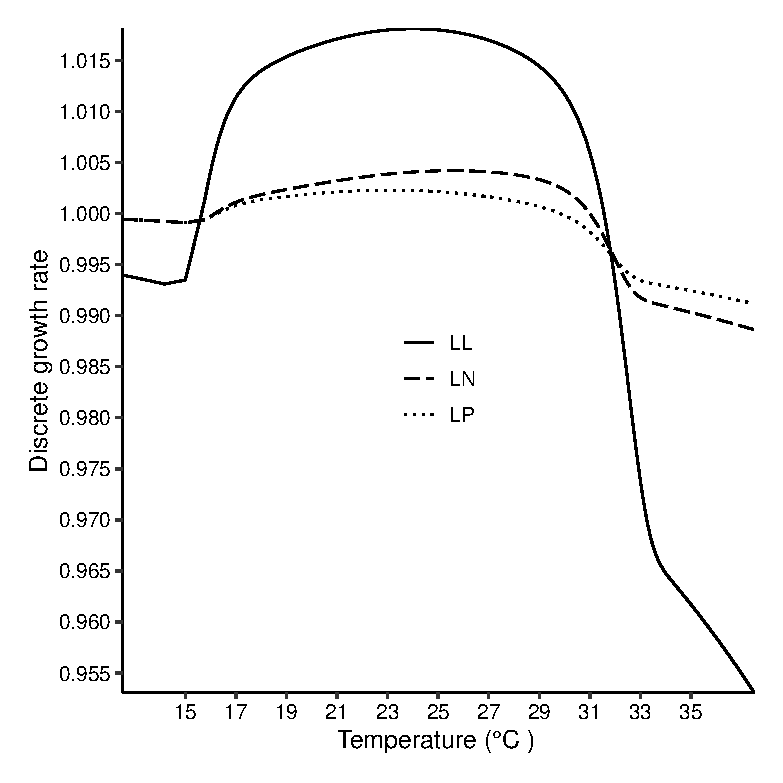
\includegraphics[width=0.7\linewidth]{LNLP}
	\caption{Discrete growth rate as a function of temperature}
	\label{fig:tsetseflowchat3}
\end{figure}





\begin{figure}[hbt!]
	\centering
	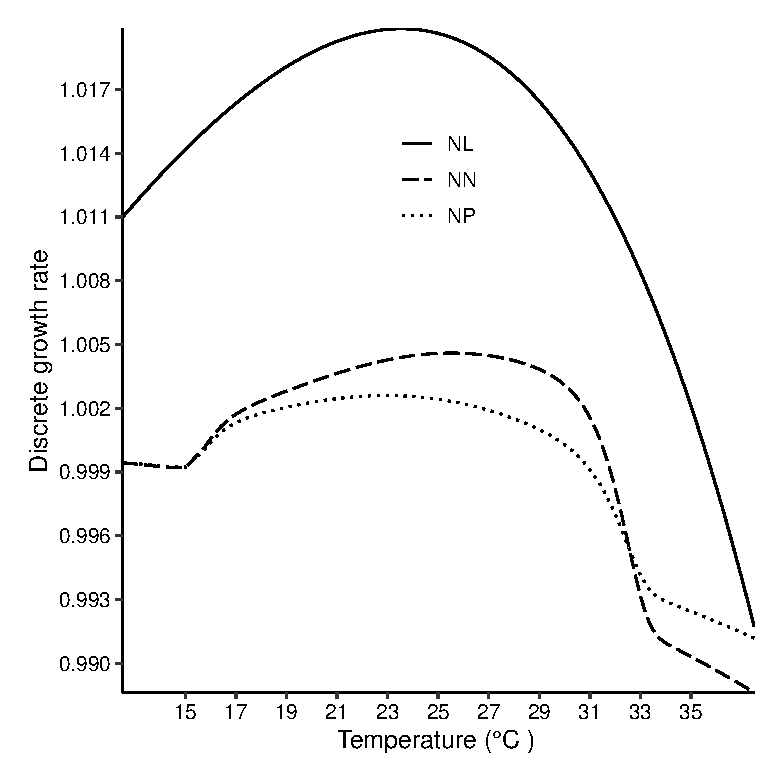
\includegraphics[width=0.7\linewidth]{NLNP}
	\caption{Discrete growth rate as a function of temperature}
	\label{fig:tsetseflowchat3}
\end{figure}





\begin{figure}[hbt!]
	\centering
	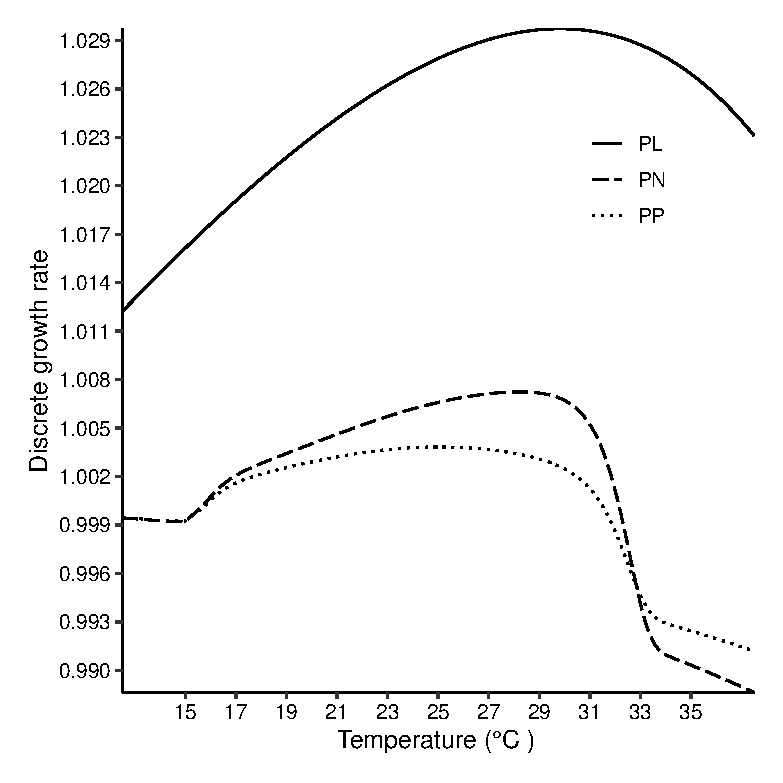
\includegraphics[width=0.7\linewidth]{PLPP}
	\caption{Discrete growth rate as a function of temperature}
	\label{fig:tsetseflowchat3}
\end{figure}

\newpage 
\section*{Possible way forward?} 

\begin{itemize}  
\item  We can estimate the growth rate $\lambda$ for a year (with annual average temperature). 

\item We can then use the temperature data for the Zambezi valley of Zimbabwe to estimate $\lambda$ for tsetse population over the past years. If our results are meaningful, we can proceed by estimating  $\lambda$ to assess tsetse population growth rate for different temperature projections. We can ask questions like, if the annual average   temperature continues to increase at the present rate, at what year will $\lambda < 1$ Or could the values of $\lambda$ explain the decline in tsetse population in the last few years, in the Zambezi valley of Zimbabwe? 
\end{itemize}


\section*{References}
\begin{enumerate} 
\item 	Are EB, Hargrove JW. Dushoff J (2019). Insect demography: does it matter if we count babies or mummies? Journal of mathematical biology (in prep).

\item 	Are EB, Hargrove JW. (2019). Extinction probabilities, times to extinction, basic reproduction number and growth rates for tsetse (Glossina spp) populations as a function of temperature. PLOS Neglected Tropical Diseases  (under review).


\end{enumerate}

\end{document}
